\documentclass[final]{IEEEtran}
\usepackage[dvips]{graphicx}
\usepackage{amsmath,amssymb}
\usepackage{array}
\usepackage{diagbox}
\usepackage{url}
\usepackage{multirow}
\usepackage[utf8]{inputenc}
\usepackage{supertabular}
\usepackage{marvosym}
\usepackage[]{algorithm2e}
\usepackage{bbm}
\usepackage{tikz}
\usepackage{tikzscale}
\usepackage{pgf}
\usetikzlibrary{calc,decorations.pathreplacing,positioning,shadows,backgrounds,arrows.meta}
\DeclareUnicodeCharacter{20AC}{\EUR{}}

\allowdisplaybreaks

% avoid overflowing urls
\expandafter\def\expandafter\UrlBreaks\expandafter{\UrlBreaks%  save the current one
  \do\a\do\b\do\c\do\d\do\e\do\f\do\g\do\h\do\i\do\j%
  \do\k\do\l\do\m\do\n\do\o\do\p\do\q\do\r\do\s\do\t%
  \do\u\do\v\do\w\do\x\do\y\do\z\do\A\do\B\do\C\do\D%
  \do\E\do\F\do\G\do\H\do\I\do\J\do\K\do\L\do\M\do\N%
  \do\O\do\P\do\Q\do\R\do\S\do\T\do\U\do\V\do\W\do\X%
  \do\Y\do\Z}

\newcommand\mycommfont[1]{\small\ttfamily{#1}}
\SetCommentSty{mycommfont}

\newcommand{\Tau}{\mathrm{T}}

\begin{document}

\title{Achieving emission reduction goals: Long-term power system expansion under short-term operational uncertainty}
\author{Authors here}
\maketitle

\begin{abstract}
Abstract here
\end{abstract}
\begin{IEEEkeywords}
Emission reduction, generation expansion, robust optimization, stochastic programming, transmission expansion
\end{IEEEkeywords}

\section{Introduction}

% introduction
Most nations have ratified the Paris agreement that aims at capping the increase in the global average temperature by lowering greenhouse gas (GHG) emissions, for example \cite{Paris_agreement}. To this end, there are nation-level policies that set speficic goals for GHG emission reductions through increasing the share of renewable energy, for example \cite{EU_climate_action}. However, integrating large investments in variable renewable energy sources (vRES) such as wind and solar power to existing power systems is likely to require significant investments in transmission capacity as well as to dispatchable RES generation technologies (e.g. hydro and biomass) and storage to guarantee the power system adequacy and security \cite{Zappa}.

% what this paper is about
Consequently, in this paper, we consider the Generation and Transmission Expansion Planning (G\&TEP) problem with the objective of reducing GHG emissions under uncertain demand and vRES generation. More specifically, we employ a tri-level model representing two stages in which the first stage and level consider a multi-year investment horizon for vRES while at the second stage, the second level uses robust optimization to choose a worst-case demand for the third level that minimizes multi-period power system operation costs under a set of vRES generation scenarios. This combination of robust optimization and stochastic programming in two stages is called stochastic adaptive robust optimization (SARO) \cite{Baringo2018}. This framework allows us to study what vRES and transmission line investments are required to meet long-term GHG emission reduction goals while meeting operational adequacy under random and worst-case perturbations in the short-term.

% literature review

% GTEP
Similar tri-level framework is employed for the G\&TEP problem in \cite{Minquez, Moreira, Baringo2018} but without the 1st and 3rd level time dimensions and a goal for GHG emission reduction. \cite{Li, Roldan} consider multiple periods at both levels but they do not focus on GHG emission reduction and use a different decomposition technique. Also, the G\&TEP problem has been studied extensively in single- (\cite{Lopez, Dominguez, Munoz}) and bi-level settings (\cite{Zhang, Pisciella, Maurovich}).

% Alternative solution methods
By contrast, \cite{Barati} consider a multi-period G&TEP problem but.

% Fully renewable
Likewise, approaches for GHG emission reduction in the energy system have been studied extensively. \cite{Hansen}, \cite{Blakers}, \cite{Colbertaldo}, and \cite{Esteban} explore the long-term plan toward a fully renewable power system in Germany, Australia, California, and Japan respectively. They all find that significant amount of vRES generation needs to be complemented with dispatchable RES generation as well as storage technologies. By contrast, \cite{Chen, Palmintier} study power system expansion with detailed short-term power system operations under constraints on GHG emissions and the share of RES generation. In particular, they find that omitting short-term flexibility constraints such as ramping constraints leads to sub-optimal expansion plans and even power systems unable to meet demand.

% central planning
Typically, the G&TEP problem is solved from the perspective of a central planner such as the transmissions system operator (TSO). Although transmission investments are often made by such a central planner, the generation investments are usually made by independent market participants \cite{Baringo2018}. However, the central planner may use incentive policies to encourage investment into certain generation units \cite{Zhou, Das}. Nevertheless, \cite{Jin, Roh, Pozo} consider multiple companies investing in generation but this leads to problems with multiple equilibria which require custom solution algorithms, possibly with computationally expensive linearization schemes.

% Other relevant work...


% contributions summarized in more detail


% paper organization
This remaining of this paper is organized as follows. Section \ref{section_problem_description} presents the mathematical formulation of our SARO problem. Section \ref{section_case_study} presents a realistic case study and its results. Finally, Section \ref{section_conclusions} provides conclucions.

\section{Problem description}
\label{section_problem_description}

\subsection{Notation}

\begin{supertabular}{p{1.5cm} p{6.5cm}}
	\multicolumn{2}{l}{\textbf{Indices}} \\
	$n$ 			& node \\
	$u$ 			& generation unit \\
	$\ell$ 		& transmission line \\
	$o$ 			& operating condition \\
	$t$ 			& time step in the master problem \\
	$\tau$ 		& time step in the subproblem \\
	$\nu$ 		& iteration in the column-and-constraint algorithm \\
	\multicolumn{2}{l}{\textbf{Sets}} \\
	$\Psi^G$ 					& existing generation units \\
	$\Psi^L$ 						& existing transmission lines \\
	$\Psi^{L,AC}$ 						& existing AC transmission lines \\
	$\Psi^{G,H}$ 				& existing hydro units \\
	$\Psi^{G+}$				& candidate generation units \\
	$\Psi^{L+}$ 				& candidate transmission lines \\
	$\Psi_n^G$ 					& existing and candidate generation units at node $n$ \\
	$\Phi^{L1/L2/L3}$		& 1st/2nd/3rd level decision variables \\
	$\Omega^M$ 					& master problem decisions variables \\
	$\Omega^S$ 					& subproblem decision variables \\
	$\Omega$						& uncertainty set \\
	$\Xi$								& feasibility set \\
	$r(\ell) / s(\ell)$ & receiving/sending-end node of line $\ell$ \\
	$\Tau^0$ 						& first subproblem time step within each master problem time step \\
	$\Tau^{-1}$ 					& last subproblem time step within each master problem time step \\
	$\Tau^{ramp}$ 			& subproblem time steps in which the ramp constraints are considered \\
	\multicolumn{2}{l}{\textbf{Parameters}} \\
	$P$ 									& normalize investment cost to operation cost level \\
	$W_o$ 												& the weight of operating condition $o$ \\
	$D$ 								& demand growth factor \\
	$\tilde{D}_{\tau, n}$ 				& nominal demand at node $n$ in period $\tau$ (MWh) \\
	$\hat{D}_{\tau, n}$ 					& demand increase at node $n$ in period $\tau$ (MWh) \\
	$E_{t}$ 											& emission target in period $t$ (tonne) \\
	$R$ 													& discount factor \\
	$C^x_{t, u}$ 							& investment cost per 1 MW of candidate unit $u$ in period $t$ (€) \\
	$C^y_{t, \ell}$ 			& investment cost of building candidate transmission line $\ell$ in period $t$ (€) \\
	$C^g_{o, \tau, u}$ 			& generation cost of unit $u$ in condition $o$ in period $\tau$ (€/MWh) \\
	$A_{o, t, u}$ 				& availability of unit $u$ in condition $o$ in period $\tau$ (\%) \\
	$G^{inv, max}_{u}$ 				& maximum invested capacity in candidate unit $u$ (MW) \\
	$G^{max}_{o, \tau, u}$ 				& maximum generation of unit $u$ in condition $o$ in period $\tau$ (MWh) \\
	$G^{ramp,max}_{o, \tau, u}$		& maximum ramp up of unit $u$ in condition $o$ in period $\tau$ (MWh) \\
	$G^{ramp,min}_{o, \tau, u}$		& maximum ramp down of unit $u$ in condition $o$ in period $\tau$ (MWh) \\
	$G^{emission}_{o, \tau, u}$	& emission rate of unit $u$ in condition $o$ in period $\tau$ (tonne/MWh) \\
	$S^0_{o, \tau, u}$ 		& initial storage level of hydro unit $u$ in condition $o$ in period $\tau$ (MWh) \\
	$S^{max}_{o, \tau, u}$ & maximum final storage level of hydro unit $u$ in condition $o$ in period $\tau$ (MWh) \\
	$S^{min}_{o, \tau, u}$ & minimum final storage level of hydro unit $u$ in condition $o$ in period $\tau$ (MWh) \\
	$I_{o, \tau, u}$ 							& inflow to hydro unit $u$ in condition $o$ in period $\tau$ (MWh) \\
	$F^{max}_{o, \tau, \ell}$			& maximum flow on line $\ell$ in condition $o$ in period $\tau$ (MWh) \\
	$F^{min}_{o, \tau, \ell}$			& minimum flow on line $\ell$ in condition $o$ in period $\tau$ (MWh) \\
	$B_\ell$ 											& susceptance of line $\ell$ (1/\Omega) \\
	$\Lambda^w$ 									& demand uncertainty budget \\
	$\Lambda^{min/max}$ 					& minimum/maximum price in the exchange (€/MWh) \\
	\multicolumn{2}{l}{\textbf{Binary variables}} \\
	$\hat{y}_{t, \ell}$ 	& equals 1 if investment is made into candidate transmission line $\ell$ in period $t$ \\
	$y_{t, \ell}$               & equals 1 if candidate transmission line $\ell$ is operational in period $t$ \\
	$w_n$                       & equals 1 if demand is increased from the nominal level at node $n$ \\
	\multicolumn{2}{l}{\textbf{Continuous variables}} \\
	$\hat{x}_{t, u}$           & new capacity of candidate generation unit $u$ built in period $t$ (MW) \\
	$x_{t, u}$                 & total built capacity of candidate generation unit $u$ in period $t$ (MW) \\
	$d_{\tau, n}$ 							& uncertain demand at node $n$ in period $\tau$ (MWh) \\
	$z_{o, \tau, n}$ 				& auxiliary variables for linearizing $\lambda_{o, \tau, n} d_{\tau, n}$ (€) \\
	$\lambda_{o, \tau, n}$					& price in condition $o$ at node $n$ in period $\tau$ (€/MWh) \\
	$\tilde{\lambda}_{o, \tau, n}$ 	& auxiliary variables for linearizing $\lambda_{o, \tau, n} d_{\tau, n}$ (€) \\
	$f_{o, \tau, \ell}$			& transmission flow in line $\ell$ in condition $o$ in period $\tau$ (MWh) \\
	$\delta_{o, \tau, n}$ 				& voltage angle at node $n$ in condition $o$ in period $\tau$ (rad) \\
	$g_{o, \tau, u}$ 					& generation at unit $u$ in condition $o$ in period $\tau$ (MWh) \\
	$s_{o, \tau, u}$ 						& storage at hydro unit $u$ in condition $o$ in period $\tau$ (MWh) \\
	$\bar{\beta}_{o, \tau, u}$ & dual variable for maximum generation of unit $u$ in condition $o$ in period $\tau$ (€/MWh) \\
	$\bar{\beta}_{o, \tau, u}^{ramp}$ & dual variable for maximum ramp up of unit $u$ in condition $o$ in period $\tau$ (€/MWh) \\
	$\underline{\beta}_{o, \tau, u}$ & dual variable for minimum generation of unit $u$ in condition $o$ in period $\tau$ (€/MWh) \\
	$\underline{\beta}_{o, \tau, u}^{ramp}$	& dual variable for maximum ramp down of unit $u$ in condition $o$ in period $\tau$ (€/MWh) \\
	$\beta_{o, t}^{emission}$ & dual variable for maximum emissions in condition $o$ in period $t$ (€/MWh) \\
	$\phi_{o, \tau, u}^{0}$ & dual variable for initial storage level of hydro unit $u$ in condition $o$ in period $\tau$ (€/MWh) \\
	$\underline{\phi}_{o, \tau, u}$ & dual variable for minimum storage of hydro unit $u$ in condition $o$ in period $\tau$ (€/MWh) \\
	$\phi_{o, \tau, u}$ & dual variable for storage level of hydro unit $u$ in condition $o$ in period $\tau$ (€/MWh) \\
	$\bar{\phi}_{o, \tau, u}^{-1}$ & dual variable for maximum final storage level of hydro unit $u$ in condition $o$ in period $\tau$ (€/MWh) \\
	$\underline{\phi}_{o, \tau, u}^{-1}$ & dual variable for minimum final storage level of hydro unit $u$ in condition $o$ in period $\tau$ (€/MWh) \\
	$\mu_{o, \tau, \ell}$ 	& dual variable for flow in AC line $\ell$ in condition $o$ in period $\tau$ (€/MWh) \\
	$\bar{\mu}_{o, \tau, \ell}$	& dual variable for maximum flow in line $\ell$ in condition $o$ in period $\tau$ (€/MWh) \\
	$\underline{\mu}_{o, \tau, \ell}$ & dual variable for minimum flow in line $\ell$ in condition $o$ in period $\tau$ (€/rad) \\
	$\bar{\mu}^{va}_{o, \tau, n}$ & dual variable for maximum voltage angle at node $n$ in condition $o$ in period $\tau$ (€/rad) \\
	$\underline{\mu}^{va}_{o, \tau, n}$ & dual variable for minimum voltage angle at node $n$ in condition $o$ in period $\tau$ (€/rad) \\
	$\mu^{ref}_{o, \tau}$ & dual variable for reference node voltage angle in condition $o$ in period $\tau$ (€/MWh) \\
	$\theta$ 	& auxiliary variable for the column-and-constraint master problem objective function (€)
\end{supertabular}

\subsection{Stochastic robust optimization problem}

The stochastic robust optimization problem is

\begin{align}
&\label{saro_obj} \underset{\Phi^{L1}}{\text{min}} \, P \sum\limits_{t} R^{-t} \left[ \sum\limits_{u \in \Psi^{G+}} C^x_{t, u} \hat{x}_{t, u} + \sum\limits_{\ell \in \Psi^{L+}} C^y_{t, \ell} \hat{y}_{t, \ell} \right] +  \\
&\underset{\Phi^{L2} \in \Omega}{\text{max}} \quad \underset{\Phi^{L3} \in \Xi}{\text{min}} \sum\limits_o W_o \sum\limits_{\tau} R^{-t(\tau)} \sum\limits_{u} C^g_{o, \tau, u} g_{o, \tau, u} \\
&\text{subject to} \nonumber \\
&\label{master_constraint_first} x_{t, u} = \sum\limits_{t' = 1}^{t} \hat{x}_{t', u} 	\quad \forall t, u \in \Psi^{G+} \\
&x_{t, u} \leq G^{inv, max}_u \quad \forall t, u \in \Psi^{G+} \\
&\label{master_constraint_last} y_{t, \ell} = \sum\limits_{t' = 1}^{t} \hat{y}_{t', \ell} 	\quad \forall t, \ell \in \Psi^{L+}
\end{align}
where $\Phi^{L1} = \{ \hat{x}_{t, u}, x_{t, u} \forall t, u \in \Psi^{G+}, \hat{y}_{t, \ell}, y_{t, \ell} \forall t, \ell \in \Psi^{L+} \}$, $\Phi^{L2} = \{ d_{\tau, n} \, \forall \tau, n, w_{n} \, \forall n \}$, and $\Phi^{L3} = \{ g_{o, \tau, u} \, \forall o, \tau, u, s_{o, \tau, u} \, \forall o, \tau, u \in \Psi^{G, H}, f_{o, \tau, \ell} \, \forall o, \tau, \ell, \delta_{o, \tau, n} \, \forall o, \tau, n \}$. The uncertainty set $\Omega$ is given by
\begin{align}
\Omega = \{ &d_{\tau, n} = D^{-t(\tau)} (\tilde{D}_{\tau, n} + w_n \hat{D}_{\tau, n}) & \forall \tau, n \nonumber \\
&\label{uncertainty_set}\sum\limits_n w_{n} \leq \Lambda^w \}.
\end{align}

Given the optimal values $x_{t, u}^* \, \forall t, u \in \Psi^{G+}$, $y_{t, \ell}^* \, \forall t, \ell \in \Psi^{L+}$, and $d_{\tau, n}^* \, \forall \tau, n$, the feasibility set $\Xi(g_{o, \tau, u}, s_{o, \tau, u}, f_{o, \tau, \ell}, \delta_{o, \tau, n})$ is
\begin{align}
\{ &\sum\limits_{u \in \Psi^G_{n}} g_{o, \tau, u} - \sum\limits_{\ell | s(\ell) = n} f_{o, \tau, \ell} + \nonumber \\
&\sum\limits_{\ell | r(\ell) = n} f_{o, \tau, \ell} = d_{\tau, n}^* \quad \forall o, \tau, n\\
&0 \leq g_{o, \tau, u} \leq A_{o, t, u} G_{o, \tau, u}^{max} \quad \forall o, \tau, u \in \Psi_n^G \\
&0 \leq g_{o, \tau, u} \leq A_{o, t, u} x_{t(\tau), u}^* \quad \forall o, \tau, u \in \Psi_n^{G+} \\
&G^{ramp,min}_{o, \tau, u} \leq g_{o, \tau + 1, u} - g_{o, \tau, u} \quad \forall o, \tau \in \Tau^{ramp}, u \\
&g_{o, \tau + 1, u} - g_{o, \tau, u} \leq G^{ramp,max}_{o, \tau, u} \quad \forall o, \tau \in \Tau^{ramp}, u \\
&\sum\limits_{\tau \in t} \sum\limits_{u} g_{o, \tau, u} G^{emissions}_{o, \tau, u} \leq E_{t} \quad \forall o, t \\
&s_{o, \tau, u} \geq 0 \quad \forall o, \tau, u \in \Psi^{G, H} \\
&s_{o, \tau, u} = S^0_{o, \tau, u} \quad \forall o, \tau \in \Tau^0, u \in \Psi^{G, H} \\
&s_{o, \tau + 1, u} = s_{o, \tau, u} - g_{o, \tau, u} + I_{o, \tau, u} \, \, \forall o, \tau \in \Tau^{ramp}, u \in \Psi^{G, H} \\
&S^{min}_{o, \tau, u} \leq s_{o, \tau, u} \leq S^{max}_{o, \tau, u} \quad \forall o, \tau \in \Tau^{-1}, u \in \Psi^{G, H} \\
&f_{o, \tau, \ell} = B_\ell (\delta_{o, \tau, s(\ell)} - \delta_{o, \tau, r(\ell)}) \quad \forall o, \tau, \ell \in \Psi^L \\
&F_{o, \tau, \ell}^{min} \leq f_{o, \tau, \ell} \leq F_{o, \tau, \ell}^{max} \quad \forall o, \tau, \ell \in \Psi^L \\
&F_{o, \tau, \ell}^{min} y_{t(\tau), \ell}^* \leq f_{o, \tau, \ell} \leq F_{o, \tau, \ell}^{max} y_{t(\tau), \ell}^* \quad \forall o, \tau, \ell \in \Psi^{L+} \\
&-\pi \leq \delta_{o, \tau, n} \leq \pi \quad \forall o, \tau, n \\
&\delta_{o, \tau, 0} = 0 \quad \forall o, \tau \}
\end{align}
where the notation $t(\tau)$ indicates to which master problem time step $t$ the subproblem time step $\tau$ is assigned to. Also, the notation $\tau \in t$ indicates subproblem time steps $\tau$ within a master problem time step $t$. The definition of the two different time scales and the related sets are shown in Figure \ref{fig_time_scales}. Hydro power is modeled following \cite{Debia} by assuming that each hydro power unit has one reservoir that can act as a storage. Finally, we assume that all candidate transmission lines are DC lines. This assumption reduces solution times because AC candidate lines would lead to constraints with a product of a binary and a continuous variable, which we would need to linearize.

\begin{figure}[htpb]
	%\centering
	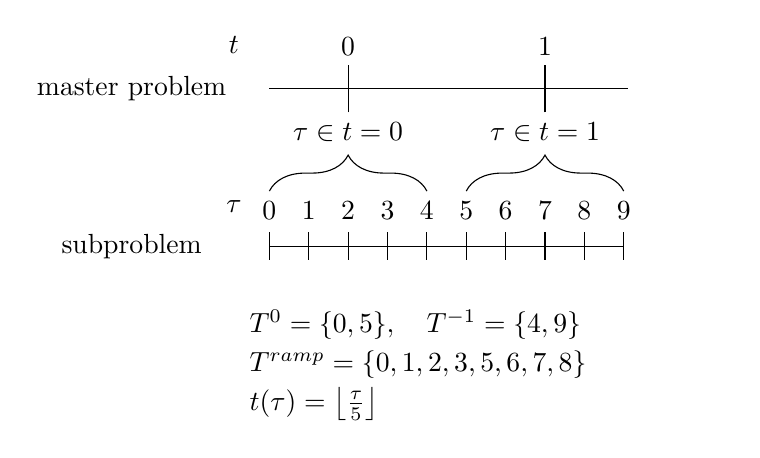
\begin{tikzpicture}
	\node at (0,0) {master problem};
	\draw (1.75,0) -- (6.3,0);
	\node at (1.3,0.55) {$t$};
	\draw (2.75,-0.3) -- (2.75,0.3) node [above] {$0$};
	\draw (5.25,-0.3) -- (5.25,0.3) node [above] {$1$};

	\draw [decorate,decoration={brace,amplitude=13pt}] (1.75,-1.3) -- (3.75,-1.3);
	\draw [decorate,decoration={brace,amplitude=13pt}] (4.25,-1.3) -- (6.25,-1.3);

	\node at (2.75,-0.55) {$\tau \in t = 0$};
	\node at (5.25,-0.55) {$\tau \in t = 1$};

	\node at (0,-2) {subproblem};
	\node at (1.3,-1.5) {$\tau$};
	\foreach \x in {0,1,2,...,9}
    {
      \coordinate (A\x) at ($(1.75,-2)+(\x*0.5cm,0)$) {};
      \draw ($(A\x)+(0,5pt)$) -- ($(A\x)-(0,5pt)$);
      \node at ($(A\x)+(0,3ex)$) {\x};
    }
	\draw (A0) -- (A9);

	\node[text width=6cm] at (4.5, -3) {$T^0 = \{ 0, 5 \}, \quad T^{-1} = \{ 4, 9 \}$};
	\node[text width=6cm] at (4.5, -3.5) {$T^{ramp} = \{ 0, 1, 2, 3, 5, 6, 7, 8 \}$};
	\node[text width=6cm] at (4.5, -4.0) {$t(\tau) = \left \lfloor{\frac{\tau}{5}}\right \rfloor $};
	\end{tikzpicture}
	\caption{$T^0$, $T^{ramp}$, $T^{-1}$, $t(\tau)$, and $\tau \in t$ in an example problem with five subproblem timesteps within each of the two master problem time steps}
	\label{fig_time_scales}
	\end{figure}

\subsection{Overview of the solution algorithm}

The problem (\ref{saro_obj})-(\ref{master_constraint_last}) is solved using column-and-constraint algorithm in which solving the first minimization problem of (\ref{saro_obj}) and solving the max-min problem of (\ref{saro_obj}) alternate. These two alternating problems are called master problem (Eqs. (\ref{master_obj})-(\ref{master_last})) and subproblem (Eqs. (\ref{sub_obj})-(\ref{sub_last})), respectively. The whole solution algorithm is summarized in Algorithm \ref{alg_algorithm}.

\begin{algorithm}
\SetAlgoLined
\DontPrintSemicolon
$\epsilon \leftarrow 10^{-6}$ \;
$LB \leftarrow -\infty$ \;
$UB \leftarrow \infty$ \;
$\nu \leftarrow 0$ \;
$d_{\tau, n, \nu} \leftarrow \tilde{D}_{\tau, n} \quad \forall \tau, n$ \;
\While{$(UB - LB) / UB \leq \epsilon$}{
	\tcp*[l]{Solve the master problem}
		Obtain $x_{t, u}^*, \hat{x}_{t, u}^* \, \forall t, u \in \Psi^{G+} \, , y_{t, \ell}^*, \hat{y}_{t, \ell}^* \, \forall t, \ell \in \Psi^{L+}$ by solving master problem in Eqs. (\ref{master_obj})-(\ref{master_last}) using $d_{\tau, n, \nu'} \quad \forall \tau, n, \nu' \leq \nu$. $LB$ is updated to the objective value of the master problem. \;

    \;

	\tcp*[l]{Solve the subproblem using Benders.}
	Obtain $w_{n} \, \forall n$ by solving Benders master problem in Eqs. (\ref{sub_obj})-(\ref{sub_last}) using the current $x_{t, u}^* \, \forall t, u \in \Psi^{G+} \, , y_{t, \ell}^* \, \forall t, \ell \in \Psi^{L+}$. $UB$ is updated to the objective value of the subproblem + $P \sum\limits_{t} R^{-t} \big( \sum\limits_{u \in \Psi^{G+}} C^x_{t, u} \hat{x}_{t, u}^* + \sum\limits_{\ell \in \Psi^{L+}} C^y_{t, \ell} \hat{y}_{t, \ell}^* \big)$ \;

    \;

    $\nu \leftarrow \nu + 1$ \;
    $d_{\tau, n, \nu} \leftarrow \tilde{D}_{\tau, n} + w_{n} \hat{D}_{\tau, n} \quad \forall \tau, n$ \;
}
\caption{Algorithm for solving the problem (\ref{saro_obj})-(\ref{master_constraint_last})}
\label{alg_algorithm}
\end{algorithm}

\subsection{Master problem}

At iteration $\nu$, we have $\Omega^{M} = \{ g_{o, \tau, u, \nu'} \, \forall o, \tau, u, \nu' \leq \nu, s_{o, \tau, u, \nu'} \, \forall o, \tau, u \in \Psi^{G, H}, \nu' \leq \nu, f_{o, \tau, \ell, \nu'} \, \forall o, \tau, \ell, \nu' \leq \nu, \delta_{o, \tau, n, \nu'} \, \forall o, \tau, n, \nu' \leq \nu \}$. Given $d_{\tau, n, \nu'}^*, \, \forall \tau, n, \nu' \leq \nu$ as input data obtained from all the previous solutions of the subproblem, the master problem at iteration $\nu$ is

\begin{align}
&\label{master_obj} \underset{\Phi^{L1}, \Omega^{M}, \theta}{\text{min}} \, P \sum\limits_{t} R^{-t} \left[ \sum\limits_{u \in \Psi^{G+}} C^x_{t, u} \hat{x}_{t, u} + \sum\limits_{\ell \in \Psi^{L+}} C^y_{t, \ell} \hat{y}_{t, \ell} \right] + \theta \\
&\text{subject to} \nonumber \\
&\text{Eqs. } (\ref{master_constraint_first}) - (\ref{master_constraint_last}) \\
&\theta \geq \sum\limits_o W_o \sum\limits_{\tau} R^{-t(\tau)} \sum\limits_{u} C_{o, \tau, u}^g g_{o, \tau, u, \nu'} \quad \forall \nu' \leq \nu \\
&\sum\limits_{u \in \Psi^G_{n}} g_{o, \tau, u, \nu'} - \sum\limits_{\ell | s(\ell) = n} f_{o, \tau, \ell, \nu'} + \nonumber \\
&\sum\limits_{\ell | r(\ell) = n} f_{o, \tau, \ell, \nu'} = d_{\tau, n, \nu'}^* \quad \forall o, \tau, n, \nu' \leq \nu \\
&0 \leq g_{o, \tau, u, \nu'} \leq A_{o, t, u} G_{o, \tau, u}^{max} \quad \forall o, \tau, u \in \Psi_n^G, \nu' \leq \nu \\
&0 \leq g_{o, \tau, u, \nu'} \leq A_{o, t, u} x_{t(\tau), u} \quad \forall o, \tau, u \in \Psi_n^{G+}, \nu' \leq \nu \\
&G^{ramp,min}_{o, \tau, u} \leq g_{o, \tau + 1, u, \nu'} - g_{o, \tau, u, \nu'} \quad \forall o, \tau \in \Tau^{ramp}, u, \nu' \leq \nu \\
&g_{o, \tau + 1, u, \nu'} - g_{o, \tau, u, \nu'} \leq G^{ramp,max}_{o, \tau, u} \quad \forall o, \tau \in \Tau^{ramp}, u, \nu' \leq \nu \\
&\sum\limits_{\tau \in t} \sum\limits_{u} g_{o, \tau, u, \nu'} G^{emissions}_{o, \tau, u} \leq E_{t} \quad \forall o, t, \nu' \leq \nu \\
&s_{o, \tau, u, \nu'} \geq 0 \quad \forall o, \tau, u \in \Psi^{G, H}, \nu' \leq \nu \\
&s_{o, \tau, u, \nu'} = S^0_{o, \tau, u} \quad \forall o, \tau \in \Tau^0, u \in \Psi^{G, H}, \nu' \leq \nu \\
&s_{o, \tau + 1, u, \nu'} = s_{o, \tau, u, \nu'} - g_{o, \tau, u, \nu'} + \nonumber \\
&\quad \quad \quad \quad \quad \, \, \, I_{o, \tau, u} \, \, \forall o, \tau \in \Tau^{ramp}, u \in \Psi^{G, H}, \nu' \leq \nu \\
&S^{min}_{o, \tau, u} \leq s_{o, \tau, u, \nu'} \leq S^{, max}_{o, \tau, u} \quad \forall o, \tau \in \Tau^{-1}, u \in \Psi^{G, H}, \nu' \leq \nu \\
&f_{o, \tau, \ell, \nu'} = B_\ell (\delta_{o, \tau, s(\ell), \nu'} - \delta_{o, \tau, r(\ell), \nu'}) \quad \forall o, \tau, \ell \in \Psi^L, \nu' \leq \nu \\
&F_{o, \tau, \ell}^{min} \leq f_{o, \tau, \ell, \nu'} \leq F_{o, \tau, \ell}^{max} \quad \forall o, \tau, \ell \in \Psi^L, \nu' \leq \nu \\
&F_{o, \tau, \ell}^{min} y_{t(\tau), \ell} \leq f_{o, \tau, \ell, \nu'} \leq F_{o, \tau, \ell}^{max} y_{t(\tau), \ell} \, \forall o, \tau, \ell \in \Psi^{L+}, \nu' \leq \nu \\
&-\pi \leq \delta_{o, \tau, n, \nu'} \leq \pi \quad \forall o, \tau, n, \nu' \leq \nu \\
&\label{master_last} \delta_{o, \tau, 0, \nu'} = 0 \quad \forall o, \tau, \nu' \leq \nu
\end{align}

\subsection{Subproblem}

For the subproblem, we set $\Omega^{S} = \{ \lambda_{o, \tau, n} \forall o, \tau, n, \bar{\beta}_{o, \tau, u}, \underline{\beta}_{o, \tau, u}, \bar{\beta}_{o, \tau, u}^{ramp}, \underline{\beta}_{o, \tau, u}^{ramp} \forall o, \tau, u,$ $\beta_{o, t}^{emission} \forall o, t,$ $\phi_{o, \tau, u}^{0} \forall o, \tau \in \Tau^0, u \in \Psi^{G, H}, \phi_{o, \tau, u} \forall o, \tau \in \Tau^{ramp}, u \in \Psi^{G, H}, \bar{\phi}_{o, \tau, u}^{-1}, \underline{\phi}_{o, \tau, u}^{-1} \forall o, \tau \in \Tau^{-1}, u \in \Psi^{G, H}, \underline{\phi}_{o, \tau, u} \forall o, \tau, u \in \Psi^{G, H}$ $\mu_{o, \tau, \ell}, \bar{\mu}_{o, \tau, \ell}, \underline{\mu}_{o, \tau, \ell} \forall o, \tau, \ell, \bar{\mu}^{va}_{o, \tau, n}, \underline{\mu}^{va}_{o, \tau, n} \forall o, \tau, n, \mu^{ref}_{o, \tau}  \forall o, \tau \}$. With $x_{t, u}^* \, \forall t, u \in \Psi^{G+}$ and $y_{t, \ell}^* \, \forall t, \ell \in \Psi^{L+}$ as input data obtained from the previous solution of the master problem, the subproblem is
\begin{align}
\label{sub_obj} \underset{\Phi^{L2}, \Omega^{S}}{\text{maximize}} &\sum\limits_o \Bigg( \sum\limits_{\tau} \Big[ \sum\limits_n \lambda_{o, \tau, n} d_{\tau, n} - \nonumber \\
&\sum\limits_{u \in \Psi^G} \bar{\beta}_{o, \tau, u} A_{o, t, u} G_{o, \tau, u}^{max} - \nonumber \\
&\sum\limits_{u \in \Psi^{G+}} \bar{\beta}_{o, \tau, u} A_{o, t, u} x_{t(\tau), u}^* - \nonumber \\
&\sum\limits_{\ell \in \Psi^L} \left( \bar{\mu}_{o, \tau, \ell} F_{o, \tau, \ell}^{max} - \underline{\mu}_{o, \tau, \ell} F_{o, \tau, \ell}^{min} \right) - \nonumber \\
&\sum\limits_{\ell \in \Psi^{L+}} \left( \bar{\mu}_{o, \tau, \ell} F_{o, \tau, \ell}^{max} - \underline{\mu}_{o, \tau, \ell} F_{o, \tau, \ell}^{min} \right) y_{t(\tau), \ell}^* - \nonumber \\
&\sum\limits_{n} \pi ( \bar{\mu}^{va}_{o, \tau, n} + \underline{\mu}^{va}_{o, \tau, n} ) \Big] + \nonumber \\
&\sum\limits_{u \in \Psi^{G, H}} \Big[ \sum\limits_{\tau \in \Tau^{0}}  \phi_{o, \tau, u}^{0} S^{0}_{o, \tau, u} + \nonumber \\
&\sum\limits_{\tau \in \Tau^{ramp}} \phi_{o, \tau, u} I_{o, \tau, u} + \nonumber \\
&\sum\limits_{\tau \in \Tau^{-1}} \left( \underline{\phi}^{-1}_{o, \tau, u} S^{min}_{o, \tau, u} - \bar{\phi}^{-1}_{o, \tau, u} S^{max}_{o, \tau, u} \right) \Big] + \nonumber \\
&\sum\limits_{\tau \in \Tau^{ramp}} \sum\limits_{u} \left( \underline{\beta}_{o, \tau, u}^{ramp} G^{ramp,min}_{o, \tau, u} - \bar{\beta}_{o, \tau, u}^{ramp} G^{ramp,max}_{o, \tau, u} \right) \nonumber \\
&\sum\limits_{t} \beta_{o, t}^{emission} E_{t} \Bigg)
\end{align}
\begin{align}
&\text{subject to} \nonumber \\
&\lambda_{o, \tau, n(u)} - \bar{\beta}_{o, \tau, u} + \underline{\beta}_{o, \tau, u} + \mathbbm{1}_{\tau \in \Tau^{ramp} \land u \in \Psi^{G, H}} \phi_{o, t, u} - \nonumber \\
&\mathbbm{1}_{\tau \notin \Tau^0} \bar{\beta}_{o, \tau - 1, u}^{ramp} + \mathbbm{1}_{\tau \notin \Tau^{-1}} \bar{\beta}_{o, \tau, u}^{ramp} + \mathbbm{1}_{\tau \notin \Tau^0} \underline{\beta}_{o, \tau - 1, u}^{ramp} - \mathbbm{1}_{\tau \notin \Tau^{-1}} \underline{\beta}_{o, \tau, u}^{ramp} - \nonumber \\
&\label{sub_constr1}G_{o, \tau, u}^{emissions} \beta_{o, t(\tau)}^{emissions} = R^{-t(\tau)} C^g_{o, \tau, u}  W_o \quad \forall o, \tau, u \\
&\mathbbm{1}_{\tau \in \Tau^0} \phi_{o, \tau, u}^{0} + \underline{\beta}_{o, \tau, u}^s - \mathbbm{1}_{\tau \notin \Tau^{-1}} \phi_{o, \tau, u} + \mathbbm{1}_{\tau \notin \Tau^0} \phi_{o, \tau - 1, u} + \nonumber \\
&\mathbbm{1}_{\tau \in \Tau^{-1}} (\underline{\phi}_{o, \tau, u} - \bar{\phi}_{o, \tau, u}) = 0 \quad \forall o, \tau, u \in \Psi^{G, H} \\
&-\lambda_{o, \tau, s(\ell)} + \lambda_{o, \tau, r(\ell)} + \mathbbm{1}_{\ell \in \Psi^{L,AC}} \mu_{o, \tau, \ell} - \nonumber \\
&\bar{\mu}_{o, \tau, \ell} + \underline{\mu}_{o, \tau, \ell} = 0 \quad \forall o, \tau, \ell \\
&-\sum\limits_{\ell \in \Psi^{L,AC} | s(\ell) = n} B_\ell \mu_{o, \tau, \ell} + \sum\limits_{\ell \in \Psi^{L,AC} | r(\ell) = n} B_\ell \mu_{o, \tau, \ell} - \nonumber \\
&\bar{\mu}^{va}_{o, \tau, n} + \underline{\mu}^{va}_{o, \tau, n} + \mathbbm{1}_{n = 0} \mu^{ref}_{o, \tau} = 0 \quad \forall o, \tau, n \\
&\label{sub_last}\text{Eqs. } (\ref{uncertainty_set}),
\end{align}
where the notation $n(u)$ indicates the node $n$ at which unit $u$ is located and $\mathbbm{1}_{cond}$ equals 1 if $cond$ is true and otherwise 0.

The subproblem can be solved directly as a MIQP. Alternatively, the subproblem can be re-formulated as an MILP by linearizing the product of a continuous and a binary variable in $\lambda_{o, \tau, n} d_{\tau, n} = \lambda_{o, \tau, n} D^{-t(\tau)} (\tilde{D}_{\tau, n} + w_n \hat{D}_{\tau, n})$ in the objective function (\ref{sub_obj}) exactly with $\lambda_{o, \tau, n} d_{\tau, n} = D^{-t(\tau)} (z_{o, \tau, n} \hat{D}_{\tau, n} + \lambda_{o, \tau, n} \tilde{D}_{\tau, n})$ and by adding the following constraints to the subproblem
\begin{align}
&\label{z_constr} z_{o, \tau, n} = \lambda_{o, \tau, n} - \tilde{\lambda}_{o, \tau, n} \quad \forall o, \tau, n \\
&\Lambda^{min} w_n \leq z_{o, \tau, n} \leq \Lambda^{max} w_n \quad \forall o, \tau, n \\
&\Lambda^{min} (1 - w_n) \leq \tilde{\lambda}_{o, \tau, n} \leq \Lambda^{max} (1 - w_n) \quad \forall o, \tau, n
\end{align}

\section{Case study: modified Nordic and Baltic network}
\label{section_case_study}

We study what investments are required to decrease the initial emissions of the Nordic and Baltic electricity system under uncertain generation and transmission parameters and worst-case realization of demand. More specifically, we use the Nordic and Baltic network and its generation, load, and transmission line data from \cite{Virasjoki} as a base.

Our case study has 10 time steps in the master problem ($t$) for making investments. For each master problem time step, we consider 24 time steps in the subproblem ($\tau$). Consequently, the subproblem has 240 time steps in total. We define variable load and wind as well as solar power data so that, for each master problem time step, we sample one day in 2014 and use data from that day. The load values increase each year by a factor of $D = 1.03$. Hydro power data such as initial storage levels ($S_{o, \tau, u}^0$) and inflows ($I_{o, \tau, u}$) have weekly granularity so these data are taken from the week that each sampled day belongs to. In addition, we modify the system by introducing 3 equally weighted ($W_o = 1/3$) operating conditions by sampling uniform noise from $\textrm{U}(-100 \textrm{ MW}, 100 \textrm{ MW})$ to all generation ($G^{max}_{o, \tau, u}$) and transmission capacities ($F^{max}_{o, \tau, \ell}$ and $F^{min}_{o, \tau, \ell}$).

A maximum 20000 MW of gas, CCGT, oil, wind and solar power can be built at each node. In addition, there is a candidate DC transmission line between each neighboring node pair with 2000 MW of capacity to both directions. The investment parameters are shown in Table \ref{table_investment_parameters}. The upper bound for emissions for each master problem time step decreases linearly from $E_{0} = 100000 \textrm{ tonne}$ to $E_{9} = 20000 \textrm{ tonne}$.

The uncertainty budget in the subproblem ($\Lambda^w$) is 2 meaning that the model can change load in maximum of 2 nodes. Each change the model makes increases load in a node for all operating conditions and subproblem time steps by $\hat{D}_{\tau, n} = 100 \textrm{ MWh}$. The linearization variables $\Lambda^{min}$ and $\Lambda^{max}$ are -1000 €/MWh and 1000 €/MWh, respectively.

\begin{table}[htpb]
\centering
\begin{tabular}{l| c} \hline
Parameter 				& Value  \\ \hline
$P$ 					& $\frac{1}{365}$ \\
$R$						& 1.1		\\
$C^x_{t, u}$ (€/MW)		& 10^6    \\
$C^x_{t, \ell}$ (€)		& 10^8	\\
\end{tabular}
\caption{Investment parameters in the case study}
\label{table_investment_parameters}
\end{table}

We solve this case study using the Algorithm \ref{alg_algorithm}. The results are show in Table \ref{table_results}.

\begin{table}[htpb]
\centering
\begin{tabular}{c c| c c c} \hline
Master problem 			& Subproblem & Objective value (€) 	& Solution time (s) 	& Iterations \\ \hline
Benders					& MIQP 				& 85719742.5196 		& 1859.21				& 3				 \\
MILP					& MIQP 				& 85719742.5196 		& 716.54				& 3				 \\
\end{tabular}
\caption{}
\label{table_results}
\end{table}

Figure \ref{fig_emissions_trajectory} shows how emissions decrease from their initial level to the final desired level during the simulation horizon and Figure \ref{fig_emissions_prices_trajectory} shows the emisssion prices. Figures \ref{fig_generation_investment} and \ref{fig_transmission_investment} show the generation and transmission investments, respectively, for achieving the final emission level.

\begin{figure}[htpb]
  \centering
  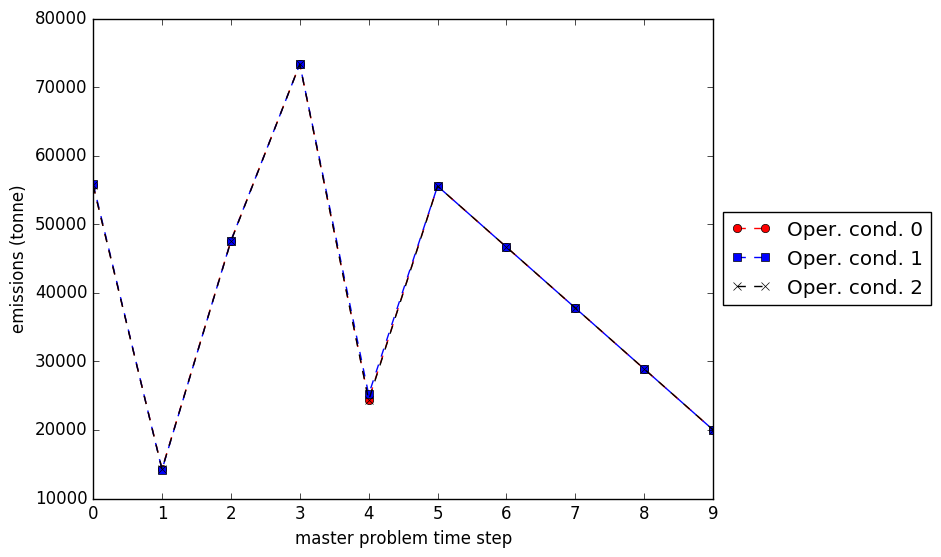
\includegraphics[width=\linewidth]{emissions_trajectory_milp_dc_miqp_dc.png}
  \caption{Decrease in emissions during the simulation horizon}
  \label{fig_emissions_trajectory}
\end{figure}

\begin{figure}[htpb]
  \centering
  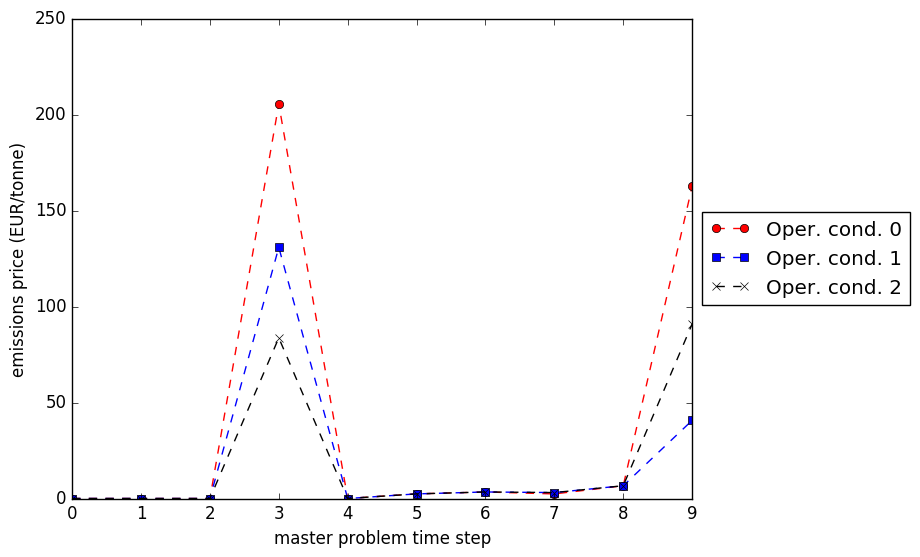
\includegraphics[width=\linewidth]{emissions_prices_trajectory_milp_dc_miqp_dc.png}
  \caption{Emissions prices during the simulation horizon}
  \label{fig_emissions_prices_trajectory}
\end{figure}

\begin{figure}[htpb]
	\centering
	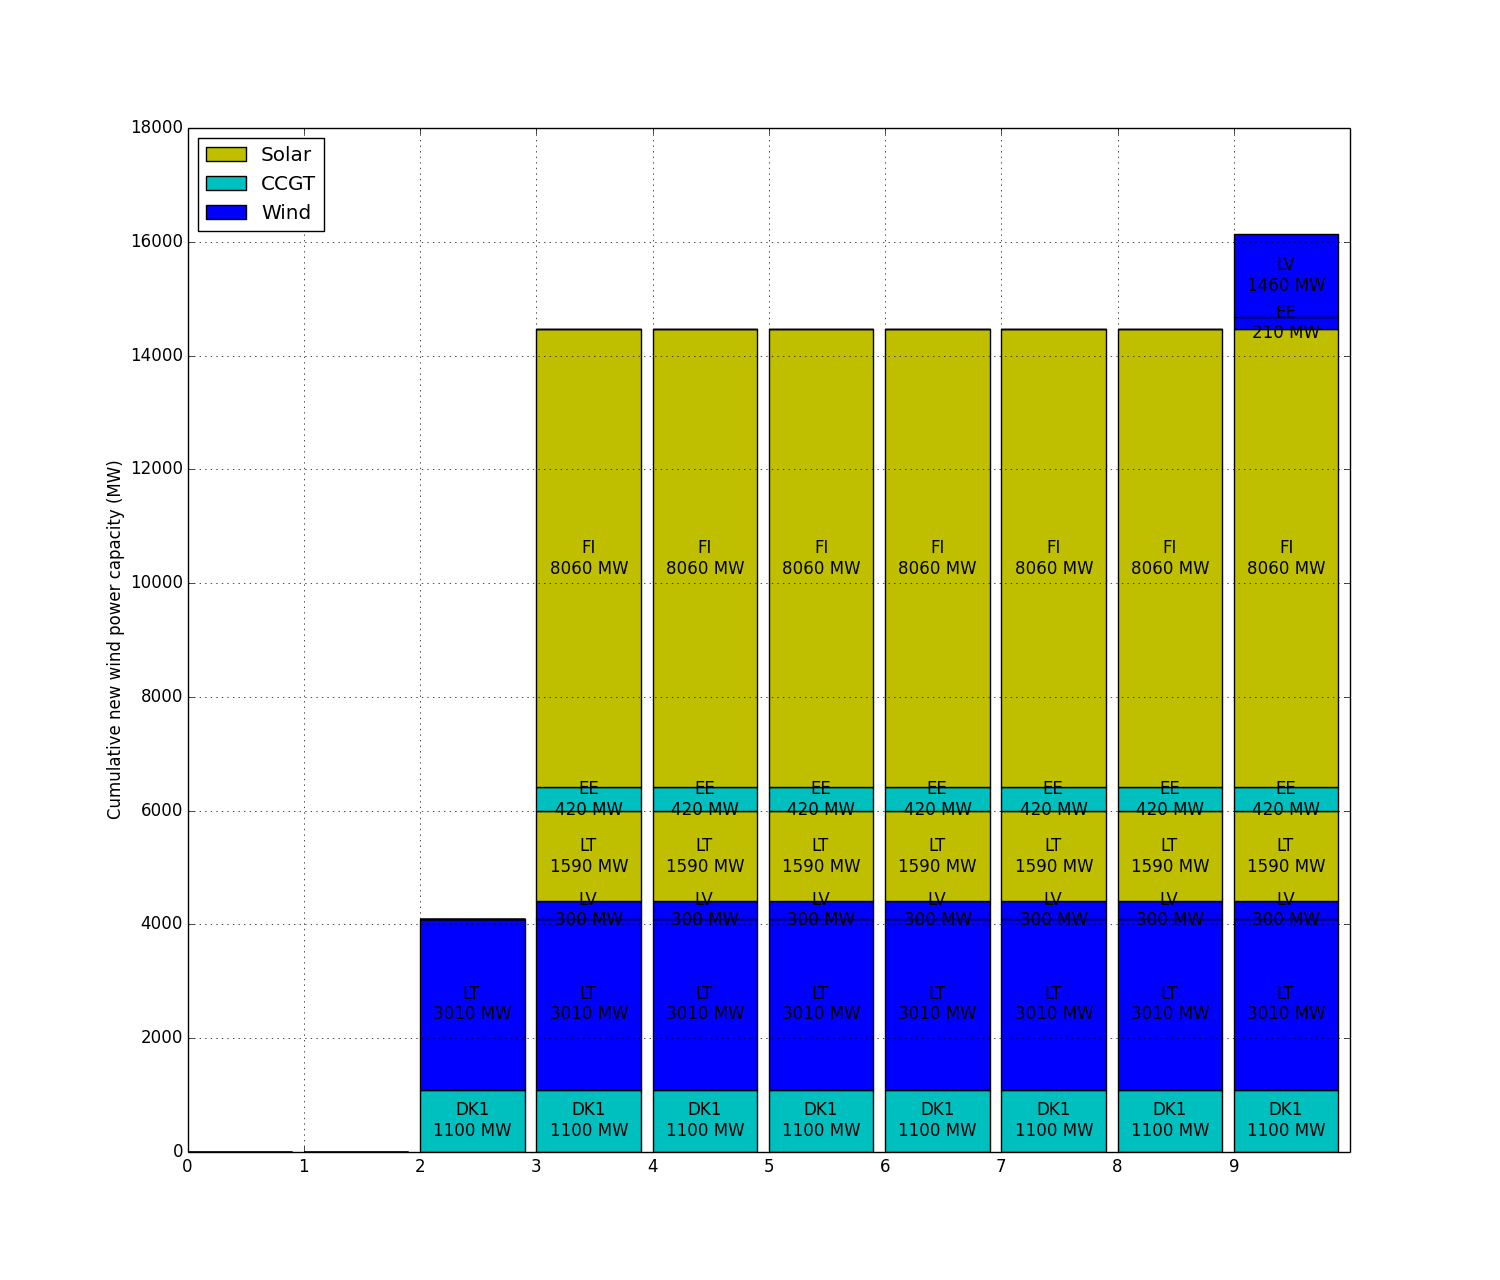
\includegraphics[width=\linewidth]{generation_investment_milp_dc_miqp_dc.png}
	\caption{Generation investments during the simulation horizon}
	\label{fig_generation_investment}
\end{figure}

\begin{figure}[htpb]
	\centering
	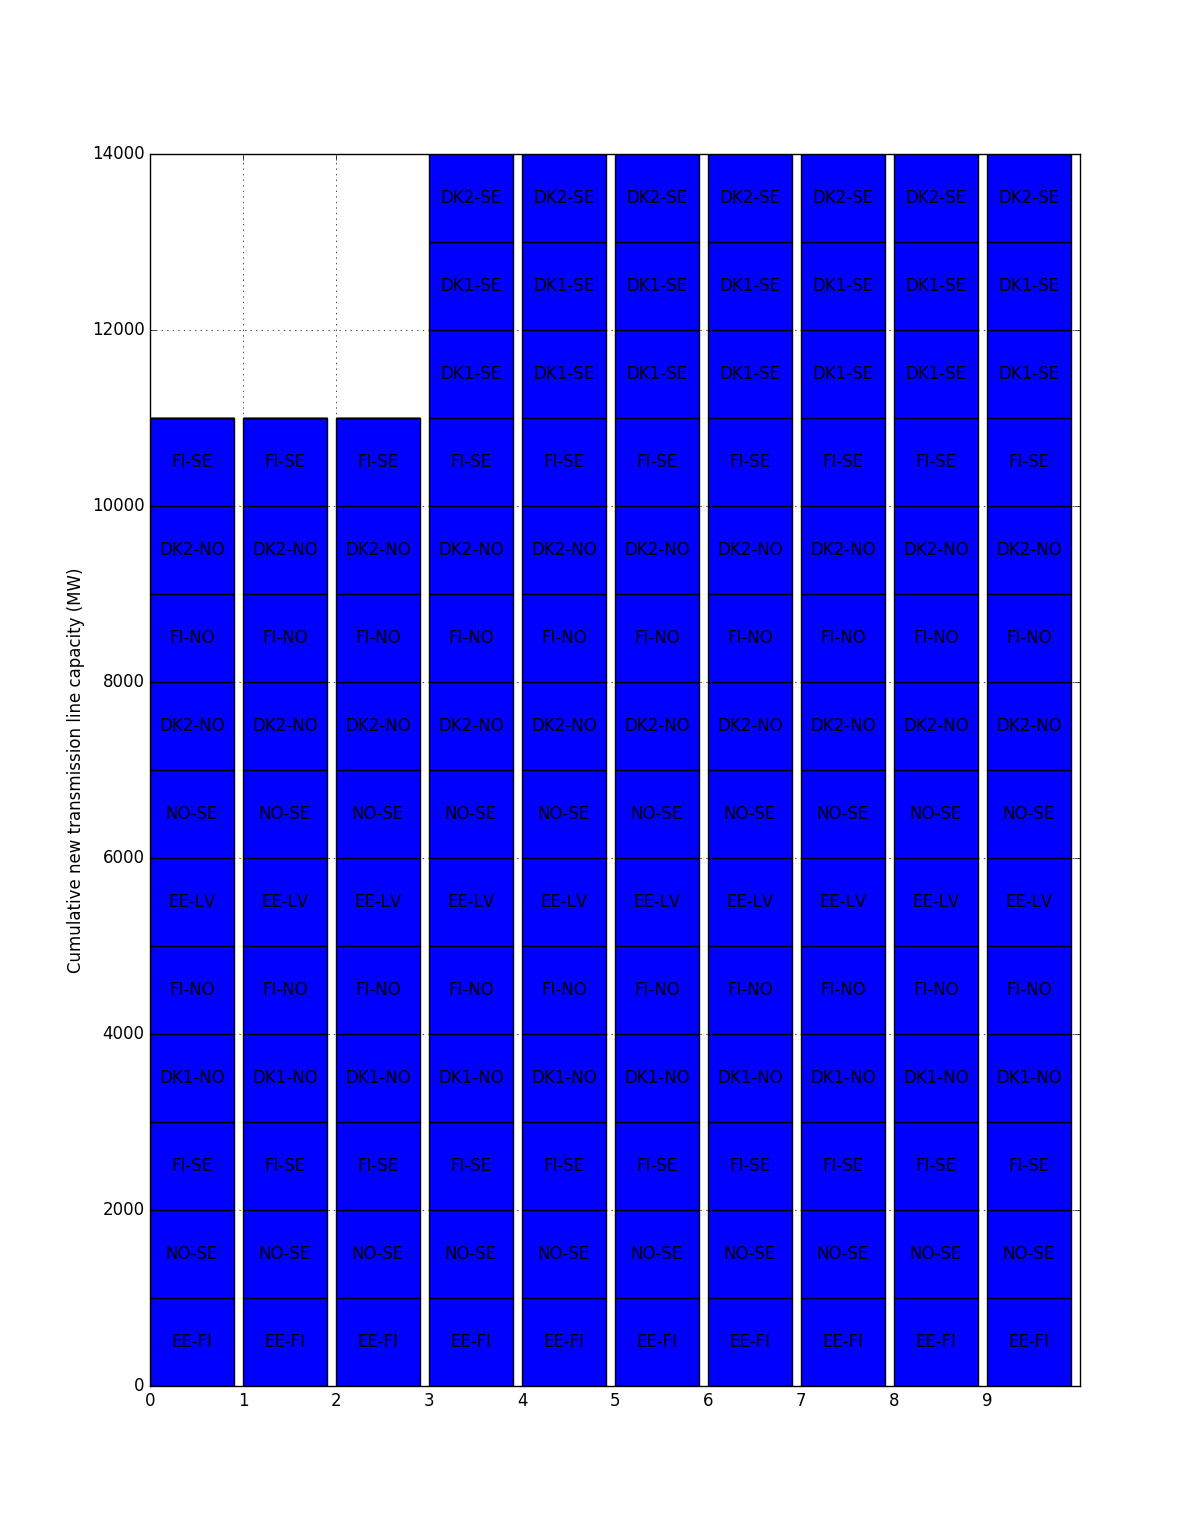
\includegraphics[width=\linewidth]{transmission_investment_milp_dc_miqp_dc.png}
	\caption{Transmission investments during the simulation horizon}
	\label{fig_transmission_investment}
\end{figure}

\section{Conclusions}
\label{section_conclusions}


\bibliographystyle{IEEEtran}
\bibliography{IEEEabrv,references}


\end{document}